\documentclass[11pt,a4paper,french]{article}
\usepackage[utf8]{inputenc}
\usepackage[T1]{fontenc}
\usepackage{babel}
\usepackage{geometry}
\usepackage{fancyhdr}
\usepackage{titlesec}
\usepackage{listings}
\usepackage{xcolor}
\usepackage{tikz}
\usetikzlibrary{positioning,arrows.meta,shadows,calc}
\usepackage{hyperref}
\usepackage{graphicx}

\geometry{margin=2.5cm}
\setlength{\headheight}{14pt}
\pagestyle{fancy}
\fancyhf{}
\chead{\textit{Éditeur de Formes Géométriques}}
\cfoot{\thepage}

\titleformat{\section}
  {\normalfont\Large\bfseries}{\thesection.}{1em}{}

\titleformat{\subsection}
  {\normalfont\large\bfseries}{\thesubsection.}{1em}{}

\lstset{
  basicstyle=\ttfamily\small,
  keywordstyle=\color{blue},
  commentstyle=\color{gray},
  stringstyle=\color{red},
  breaklines=true,
  frame=single,
  backgroundcolor=\color{white},
  language=Java
}

\title{\textbf{Éditeur de Formes Géométriques}\\
  \large{Rapport de Projet}}
\author{AMARA Kousay}
\date{Avril 2026}

\begin{document}

\maketitle

\section*{Sujet}
Micro-éditeur de figures géométriques vectorielles en Java AWT démontrant l'application de design patterns pour une architecture maintenable et extensible.

\vspace{1cm}

\section{Introduction}

J'ai conçu un éditeur vectoriel interactif en Java AWT permettant de créer, modifier, grouper et annuler des opérations sur des formes géométriques. L'objectif était de démontrer l'application de design patterns pour construire une architecture maintenable, extensible et testable.

Le sujet officiel comporte 8 cas d'utilisation. Cette version couvre l'ensemble du périmètre attendu : drag-drop de formes depuis une toolbar, groupage/dégroupage, édition des propriétés, sauvegarde de prototypes via clone, undo/redo, sauvegarde/chargement d'un document et persistance de la toolbar au redémarrage. L'implémentation s'appuie sur 20 tests unitaires.

\textbf{Contexte} : Ce projet a été réalisé en solo. L'implémentation couvre les 8 cas d'utilisation du sujet, avec une sélection multiple réalisée par \texttt{Ctrl+clics} successifs ou par rectangle de sélection.

\section{Les Six Design Patterns Appliqués}

\subsection{Composite Pattern}

Le problème était simple : comment traiter les formes individuelles et les groupes de formes de la même manière ? J'ai créé une interface \texttt{Shape} (Shape.java ligne 4) que tout implémente : Rectangle, RegularPolygon, mais aussi Group.

Group est le nœud composite. Il contient une liste d'autres shapes et implémente les mêmes opérations (move, rotate, etc.). Quand on appelle \texttt{move()} sur un groupe, l'opération s'applique récursivement à tous les enfants, même s'ils sont eux-mêmes des groupes imbriqués. Cela a éliminé le besoin de traiter les groupes différemment du reste du code.

C'est particulièrement utile pour les cas d'utilisation 2 et 3 du sujet où on doit grouper et dégrouper des formes. Un groupe peut contenir d'autres groupes sans limite.

\subsection{Prototype Pattern}

Pour la toolbar, j'avais besoin de cloner des formes avec toutes leurs propriétés. Au lieu de créer des constructeurs complexes, chaque shape implémente une méthode \texttt{clone()}.

En regardant le code : Shape.java ligne 19 définit l'interface, et chaque implémentation (Rectangle ligne 52, RegularPolygon ligne 90, Group ligne 120) retourne une copie conforme. La copie est une vraie duplication des propriétés et, dans le cas de Group, elle clone récursivement tous les enfants.

Cela simplifiait énormément le drag-drop dans la toolbar : on stocke un prototype pour chaque forme, et quand l'utilisateur la traîne, on appelle \texttt{clone()} pour créer une instance indépendante. Si l'utilisateur la remet dans la toolbar, on la clone de nouveau.

Les cas 7 et 8 s'appuient aussi sur ce mécanisme : la persistance de la toolbar sauvegarde l'ensemble des prototypes courants et les restaure au prochain démarrage via ces mêmes méthodes \texttt{clone()}.

\subsection{Command Pattern}

C'était le pattern critique du projet, celui sur lequel le sujet insistait : l'undo/redo. J'ai implémenté Command (Command.java ligne 3) comme une interface avec deux responsabilités : \texttt{execute()} pour faire l'action et \texttt{undo()} pour l'inverser.

Chaque opération dans l'éditeur est une commande concrète : AddShapeCommand, RemoveShapeCommand, MoveShapeCommand, EditShapeCommand, GroupCommand, UngroupCommand, ainsi que AddPrototypeCommand et RemovePrototypeCommand pour les actions liées à la toolbar. CommandHistory (ligne 6) gère le mécanisme avec un double-stack : une pile undo et une pile redo.

Quand l'utilisateur ajoute un premier rectangle, puis un second, puis groupe les deux, le système empile trois commandes. Quand on clique undo 3 fois, chaque commande défait son action dans l'ordre inverse. Redo refait dans le bon ordre. C'est une mécanique classique et fiable.

L'avantage est que chaque commande ne connaît que sa propre logique d'undo. Ajouter une nouvelle commande = ajouter une classe. Aucune modification à CommandHistory n'est nécessaire.

Pour le cas 7, après le chargement d'un document, \texttt{history.clear()} réinitialise les deux piles pour qu'il soit impossible d'annuler vers l'état précédent l'ouverture du fichier.

\subsection{Memento Pattern}

Le Memento capture un snapshot de l'état d'une shape : position, taille, rotation, couleur, etc. ShapeMemento (ligne 11) stocke ces propriétés.

Ce pattern est utilisé surtout dans EditShapeCommand (ligne 12). Avant que l'utilisateur modifie une shape dans le PropertyDialog, on crée un memento de l'état original. L'utilisateur édite (la shape change). Après ``OK'', on crée un second memento avec le nouvel état. Quand on undo, on restaure le memento original.

Dans cette implémentation, le memento porte lui-même la logique de restauration. La méthode \texttt{restore()} remet l'état précédent ou suivant sans exposer tous les détails internes à l'historique des commandes.

\subsection{Strategy Pattern}

J'avais un problème : PropertyDialog avait 80+ lignes de code dupliquées pour éditer Rectangle, RegularPolygon, ou Group—le même pattern (créer des champs, récupérer les valeurs, valider) mais avec des champs différents selon le type.

J'ai créé PropertyEditorStrategy (ligne 10) comme interface. La méthode \texttt{setupFields()} crée les bons champs et \texttt{applyChanges()} récupère les valeurs. Puis j'ai écrit trois implémentations : RectanglePropertyEditor, PolygonPropertyEditor, GroupPropertyEditor.

PropertyDialog délègue maintenant le travail à la bonne stratégie (choix dynamique). Cela a réduit PropertyDialog de 252 lignes à 124 lignes. Et si j'ajoute une nouvelle forme à l'avenir, je crée une nouvelle stratégie sans toucher à PropertyDialog, avec ajout du cas correspondant dans la factory.

\subsection{Observer Pattern}

Le modèle et la vue doivent rester découplés. Pour cela, j'ai implémenté un mécanisme d'observation au niveau de la scène.

\texttt{SceneListener} définit une interface de notification avec la méthode \texttt{onShapeChanged()}. La classe \texttt{Scene} maintient une liste de listeners et appelle \texttt{notifyListeners()} lors des changements de structure de la scène : ajout ou suppression de formes, réorganisation, et mise à jour de la sélection.

\texttt{WhiteboardPanel} implémente \texttt{SceneListener}. Quand il reçoit une notification, il déclenche un \texttt{repaint()} pour redessiner l'affichage.

Dans l'implémentation actuelle, ce pattern couvre donc bien les changements portés par \texttt{Scene}. En revanche, certaines modifications interactives plus fines, comme certains déplacements ou éditions appliqués directement aux formes, provoquent encore un rafraîchissement explicite côté interface. L'Observer est donc présent et utile pour découpler la scène de la vue, mais il ne couvre pas encore automatiquement toutes les mutations internes des objets métier.

Le cas 7 bénéficie aussi de l'Observer : \texttt{scene.replaceShapes()} appelle \texttt{notifyListeners()} en fin d'exécution, ce qui déclenche automatiquement le redessinage complet de la vue après chargement.

\section{Tests et Validation}

La suite de tests compte 20 tests essentiels qui couvrent les cas importants.

CommandTest contient 8 tests : chaque type de commande critique est testé individuellement, avec un test d'intégration \texttt{testCompleteUndoRedoSequence()} qui enchaîne création, groupage et déplacement de formes, validant la mécanique du double-stack, ainsi qu'un test vérifiant la restauration de l'ordre des formes après undo d'un groupage.

ModelTest contient 10 tests sur la création, le clonage, le mouvement de formes, et la hiérarchie des groupes imbriqués.

ShapePersistenceServiceTest ajoute 2 tests dédiés à la sérialisation logique : sauvegarde/rechargement de formes simples, puis sauvegarde/rechargement d'un groupe imbriqué avec conservation de la hiérarchie et des propriétés essentielles.

La couverture reste cependant centrée sur le noyau modèle/commandes. L'interface AWT, la toolbar, PropertyDialog, SelectionController et les commandes de prototypes ne sont pas testés automatiquement.

\section{Conformité aux Cas d'Utilisation}

Le sujet comporte 8 cas d'utilisation. Le projet couvre les 8 cas :

\begin{enumerate}
  \item \textbf{Drag-drop toolbar} : AddShapeCommand gère l'ajout dans la scène
  \item \textbf{Groupage} : Group et SelectionController gèrent la sélection et la création du groupe ; la sélection multiple est réalisée via des \texttt{Ctrl+clics} successifs ou par rectangle de sélection
  \item \textbf{Dégroupage} : UngroupCommand décompose le groupe et remet les formes individuelles
  \item \textbf{Édition propriétés} : EditShapeCommand + PropertyDialog ; les propriétés éditables incluent position, taille, rotation, couleur, et pour les formes simples le centre de rotation, initialisé par défaut sur le centre de la forme puis modifiable
  \item \textbf{Drag-drop vers toolbar} : \texttt{clone()} + AddPrototypeCommand pour ajouter un prototype ; suppression vers la poubelle via RemoveShapeCommand
  \item \textbf{Undo/Redo} : CommandHistory avec double-stack, cœur du système
  \item \textbf{Sauvegarde/chargement document} : boutons \texttt{Save}/\texttt{Load} dans ControlPanel ; sérialisation des formes de la scène via \texttt{ShapePersistenceService}
  \item \textbf{Persistance toolbar} : l'état des prototypes est sauvegardé à la fermeture puis restauré au démarrage
\end{enumerate}

\section{Architecture Globale}

L'architecture respecte les spécifications du sujet, notamment la séparation entre les objets gérant le rendu graphique et les objets contenant les données de la scène.

\begin{center}
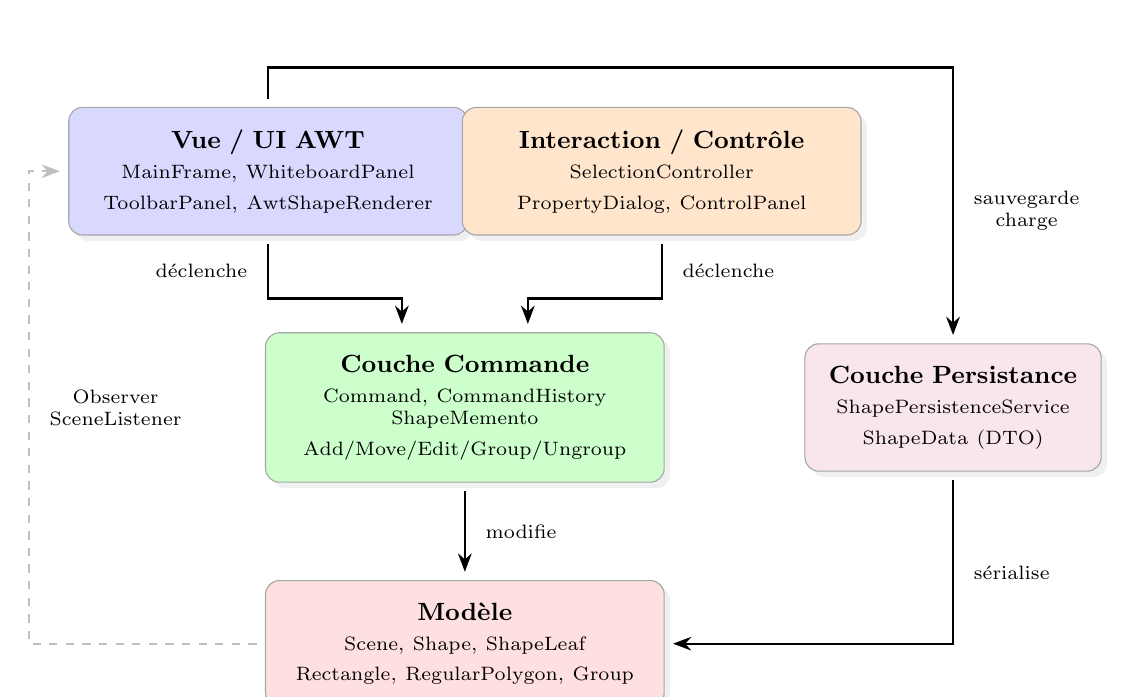
\begin{tikzpicture}[
  bloc/.style={
    draw=gray!70, rounded corners=5pt,
    text width=4.5cm, minimum height=1.6cm,
    align=center, inner sep=8pt, font=\small,
    drop shadow={opacity=0.12}
  },
  fl/.style={->, thick, >=Stealth, shorten >=3pt, shorten <=3pt}
]

  % --- Noeuds ---
  \node[bloc, fill=blue!15]   (vue)  at (-2.5, 7.0)
    {\textbf{Vue / UI AWT}\\[3pt]
     \scriptsize MainFrame, WhiteboardPanel\\ToolbarPanel, AwtShapeRenderer};

  \node[bloc, fill=orange!20] (ctrl) at ( 2.5, 7.0)
    {\textbf{Interaction / Contrôle}\\[3pt]
     \scriptsize SelectionController\\PropertyDialog, ControlPanel};

  \node[bloc, fill=green!20]  (cmd)  at ( 0.0, 4.0)
    {\textbf{Couche Commande}\\[3pt]
     \scriptsize Command, CommandHistory\\ShapeMemento\\
     \scriptsize Add/Move/Edit/Group/Ungroup};

  \node[bloc, fill=red!12]    (mod)  at ( 0.0, 1.0)
    {\textbf{Modèle}\\[3pt]
     \scriptsize Scene, Shape, ShapeLeaf\\Rectangle, RegularPolygon, Group};

  % --- Flèches ---

  % Contrôle déclenche Commandes
  \draw[fl] (ctrl.south) -- ++(0,-0.8) -| ($(cmd.north)+(0.8,0)$);
  \node[font=\scriptsize, right=4pt] at ($(ctrl.south)+(0,-0.45)$) {déclenche};

  % Vue déclenche Commandes
  \draw[fl] (vue.south) -- ++(0,-0.8) -| ($(cmd.north)+(-0.8,0)$);
  \node[font=\scriptsize, left=4pt] at ($(vue.south)+(0,-0.45)$) {déclenche};

  % Commandes modifie Modèle
  \draw[fl] (cmd.south) -- (mod.north);
  \node[font=\scriptsize, right=4pt] at ($(cmd.south)!0.5!(mod.north)$) {modifie};

  % Observer : angles droits garantis via coordinate intermédiaire
  \coordinate (obsL) at ($(mod.west)+(-3.0,0)$);
  \draw[fl, dashed, gray!50]
    (mod.west) -- (obsL) -- (obsL |- vue.west) -- (vue.west);
  \node[font=\scriptsize, align=center, right=4pt]
    at ($(obsL)!0.5!(obsL |- vue.west)$) {Observer\\SceneListener};

  % --- Couche Persistance (côté droit) ---
  \node[bloc, fill=purple!10, text width=3.2cm] (pers) at (6.2, 4.0)
    {\textbf{Couche Persistance}\\[3pt]
     \scriptsize ShapePersistenceService\\ShapeData (DTO)};

  % Vue/MainFrame → Persistance (sauvegarde/chargement, passe par-dessus les blocs)
  \draw[fl] (vue.north) -- ++(0,0.5) -| (pers.north);
  \node[font=\scriptsize, align=center, right=4pt] at (6.2, 6.5) {sauvegarde\\charge};

  % Persistance → Modèle (sérialisation)
  \draw[fl] (pers.south) |- (mod.east);
  \node[font=\scriptsize, right=4pt] at (6.2, 1.9) {sérialise};

\end{tikzpicture}
\end{center}

\noindent Ce diagramme suit la logique vue en cours et dans les corrections : une architecture par blocs, avec les dépendances principales visibles sans détailler toute l'UML des classes.

\textbf{Modèle} : Shape (interface), Rectangle, RegularPolygon, Group (composite), Scene (conteneur). Ces classes contiennent uniquement les données et la logique métier, sans rendu graphique.

\textbf{Vue / UI AWT} : MainFrame (orchestrateur, détient Scene, CommandHistory et ShapePersistenceService), WhiteboardPanel (fenêtre de dessin), ToolbarPanel (affichage des prototypes), AwtShapeRenderer (rendu graphique). Le rendu reste indépendant des données.

\textbf{Couche Commande} : Command (interface), CommandHistory (gestion undo/redo), ShapeMemento (snapshots d'état), et 8 commandes concrètes. Cela permet des opérations réversibles.

\textbf{Interaction / Contrôle} : PropertyDialog (édition des propriétés), SelectionController (logique de sélection/groupage). Ces composants orchestrent l'interaction utilisateur et déclenchent certaines modifications du modèle, directement ou via les commandes.

\textbf{Couche Persistance} : ShapePersistenceService sérialise/désérialise les formes (sérialisation Java) ; ShapeData est le DTO de transfert. Cette couche gère la sauvegarde du document (cas 7) et la persistance de la toolbar entre sessions (cas 8).

Cette organisation maintient une séparation claire des responsabilités et facilite la maintenance.

\section{Conclusion}

Ce projet a appliqué six design patterns fondamentaux :

\begin{itemize}
  \item \textbf{Composite} pour la hiérarchie de formes
  \item \textbf{Prototype} pour le clonage et la toolbar
  \item \textbf{Command} pour undo/redo
  \item \textbf{Memento} pour sauvegarder/restaurer l'état
  \item \textbf{Strategy} pour l'édition polymorphe des propriétés
  \item \textbf{Observer} pour le découplage modèle-vue
\end{itemize}

Ces patterns structurent les points les plus importants du projet : hiérarchie de formes, clonage pour la toolbar, annulation/rétablissement des actions, édition selon le type de forme, et découplage partiel entre scène et affichage. L'architecture facilite l'extension, mais certaines zones restent à adapter lorsqu'on ajoute une nouvelle forme, notamment le renderer, la factory des éditeurs, certains calculs géométriques et la sauvegarde/restauration d'état.

\section{Limites Connues}

\begin{itemize}
  \item Le format de persistance est binaire et spécifique au projet ; il n'est pas pensé pour l'interopérabilité.
  \item Le mécanisme Observer couvre surtout les changements de scène et de sélection ; certaines mises à jour restent déclenchées explicitement par l'interface.
  \item L'édition des groupes reste plus simple que celle des formes élémentaires : on édite leur centre global, leur rotation et leur échelle, mais pas un pivot distinct.
  \item L'ajout d'une nouvelle forme reste faisable, mais demande encore des modifications dans plusieurs classes transverses.
\end{itemize}

\vspace{1cm}

\noindent\textbf{Fichiers clés du projet :}

\begin{itemize}
  \item \texttt{src/main/java/model/Shape.java} (Composite + Prototype)
  \item \texttt{src/main/java/command/Command.java} et \texttt{CommandHistory.java} (Command)
  \item \texttt{src/main/java/command/ShapeMemento.java} (Memento)
  \item \texttt{src/main/java/ui/strategy/PropertyEditorStrategy.java} (Strategy)
  \item \texttt{src/main/java/model/Scene.java} (Observer)
  \item \texttt{src/main/java/persistence/ShapePersistenceService.java} (cas 7 et 8)
  \item \texttt{src/test/java/command/CommandTest.java} (tests undo/redo)
\end{itemize}

\end{document}
